\chapter{华为云资源与MindSpore框架使用方法}

\section{使用华为云计算资源}\label{sec:huawei-cloud-usage}

\subsection{创建开发环境}

我们将使用华为ModelArts平台,ModelArts是华为云提供的AI开发平台,同学们可在实名登陆后通过\url{https://www.huaweicloud.com/product/modelarts.html}, 点击管理控制台进入ModelArts管理控制台,图\ref{fig:huawei-cloud-modelart-homepage}。
\begin{figure}[htbp]
	\centering
	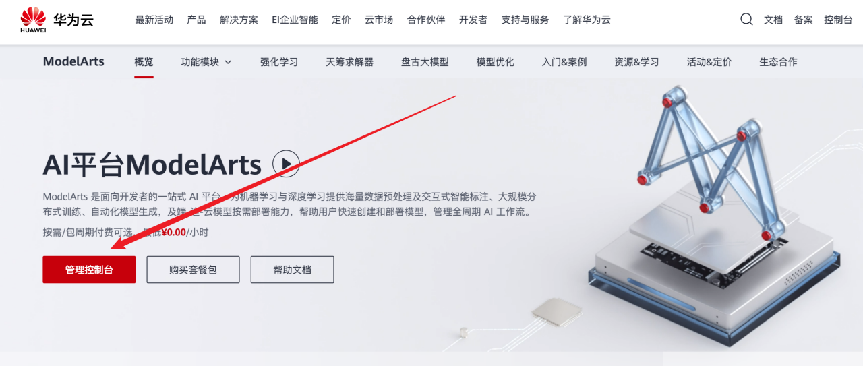
\includegraphics[width=0.7\textwidth]{figures/huawei-cloud-modelart-homepage.png}
	\caption{caption:huawei-cloud-modelart-homepage}
	\label{fig:huawei-cloud-modelart-homepage}
\end{figure}

进入管理控制台后,首先把区域切换到“北京四”,防止出现找不到资源的情况,图\ref{fig:huawei-modelarts-beijing4}。
\begin{figure}[htbp]
	\centering
	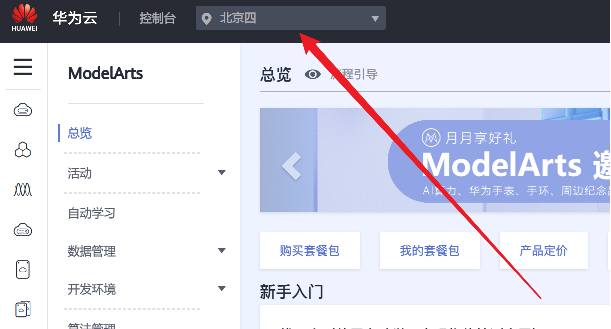
\includegraphics[width=0.7\textwidth]{figures/huawei-modelarts-beijing4.png}
	\caption{caption:huawei-modelarts-beijing4}
	\label{fig:huawei-modelarts-beijing4}
\end{figure}

从左边导航栏中进入在线开发环境,即选择开发环境-Notebook。然后点击创建按钮以创建开发环境,图\ref{fig:huawei-modelarts-notebook}。

\begin{figure}[htbp]
	\centering
	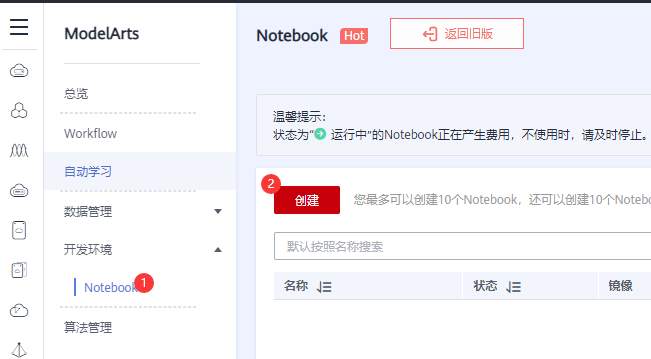
\includegraphics[width=0.7\textwidth]{figures/huawei-modelarts-notebook.png}
	\caption{caption:huawei-modelarts-notebook}
	\label{fig:huawei-modelarts-notebook}
\end{figure}


选择合适的镜像、资源规格、储存空间等,如图\ref{fig:huawei-modelarts-environment-create}所示。如需进行远程开发,请打开SSH远程开发按钮,并设置密钥对。

\begin{figure}[htbp]
	\centering
	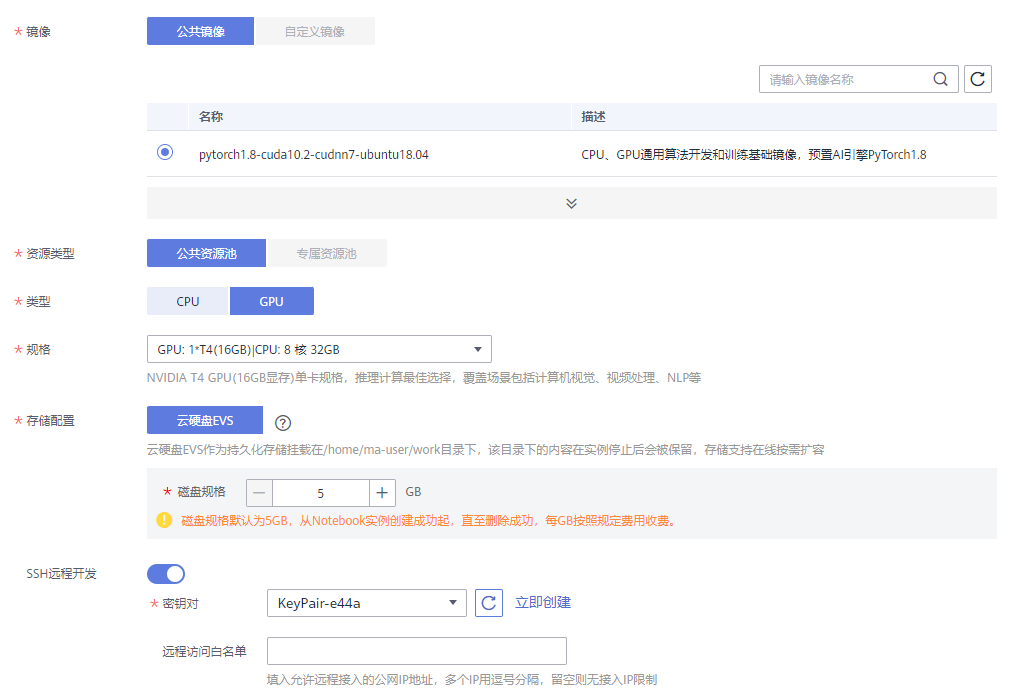
\includegraphics[width=0.7\textwidth]{figures/huawei-modelarts-environment-create.png}
	\caption{caption:huawei-modelarts-environment-create}
	\label{fig:huawei-modelarts-environment-create}
\end{figure}

如没有密钥对,需创建密钥对,点击图\ref{fig:huawei-modelarts-environment-create}中的立即创建,按照图\ref{fig:huawei-modelarts-keypair-create}所示步骤创建密钥对,并将私钥文件保存到本地。私钥文件,建议保存到 C:\textbackslash Users\textbackslash <username>\textbackslash .ssh文件夹下。

\begin{figure}[htbp]
	\centering
	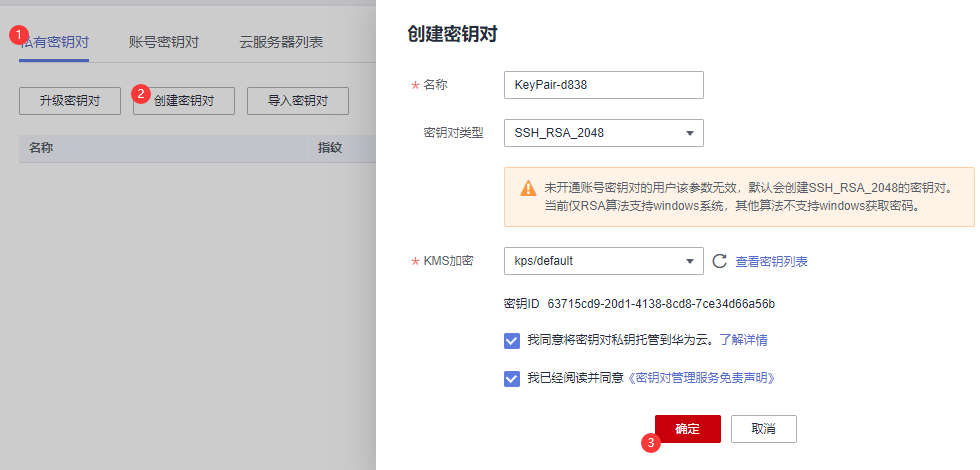
\includegraphics[width=0.7\textwidth]{figures/huawei-modelarts-keypair-create.png}
	\caption{caption:huawei-modelarts-keypair-create}
	\label{fig:huawei-modelarts-keypair-create}
\end{figure}

如此,我们便成功创建了一个开发环境,我们可以在此环境之下安装其他包,此处不再赘述。

\subsection{添加数据存储}

当有多个开发环境实例都需要使用同一个数据集时,相比每次新建实例都从本地上传,还可以选择为每一个实例都挂载同一个数据存储空间。

点击刚才创建的实例,按照图\ref{fig:huawei-modelarts-filesystem-mount}所示,点击添加数据存储,在弹出的窗口中编辑本地挂载目录,即新建的储存空间会挂在到该实例的什么地方。再选择并行文件系统,如此处为空,则点击新建并行文件系统,在新弹出的界面输入文件系统名称后点击立即创建即可。

在Notebook中挂载OBS,不适用于对挂载文件做频繁随机修改,适用于对不同挂载大小文件对象的一次保存(上传),多次读取(下载)。

\begin{figure}[htbp]
	\centering
	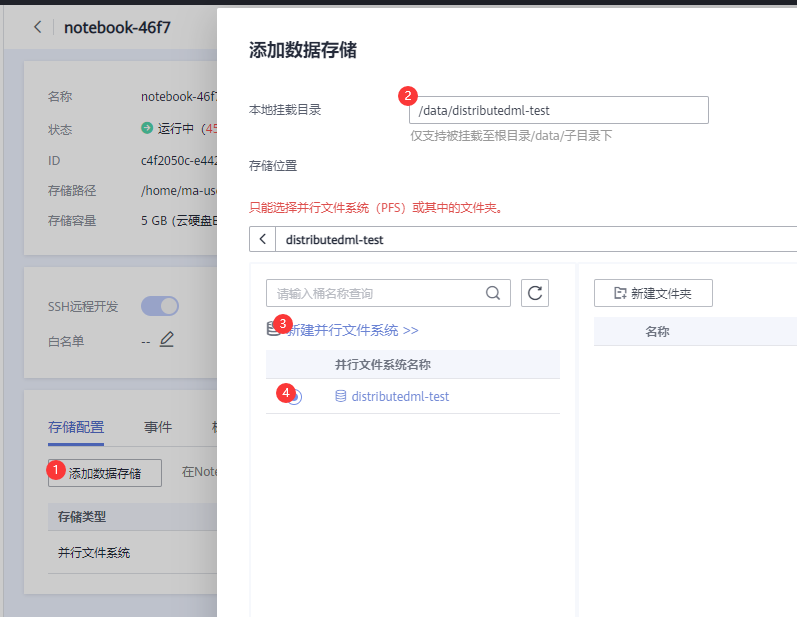
\includegraphics[width=0.7\textwidth]{figures/huawei-modelarts-filesystem-mount.png}
	\caption{caption:huawei-modelarts-filesystem-mount}
	\label{fig:huawei-modelarts-filesystem-mount}
\end{figure}

\vspace{3em}
更多问题可以参考:\url{https://support.huaweicloud.com/modelarts/index.html}

\section{MindSpore介绍}

华为开源自研AI框架{\CJKfontspec{HanaMinA}昇}思MindSpore,是一个全场景深度学习框架,旨在实现易开发、高效执行、全场景覆盖三大目标。自动微分、并行加持,一次训练,可多场景部署。支持端边云全场景的深度学习训练推理框架,主要应用于计算机视觉、自然语言处理等AI领域。

\subsection{整体介绍}

华为AI致力于构建业界最强的AI算力平台,使能千行百叶的智能化转型。华为AI的整体框架如图\ref{fig:mindspore-whole-picture}所示,其中可以看到我们在\S\ref{sec:huawei-cloud-usage}中介绍的华为ModelArts平台和MindSpore框架所处的位置。
\begin{figure}[htbp]
	\centering
	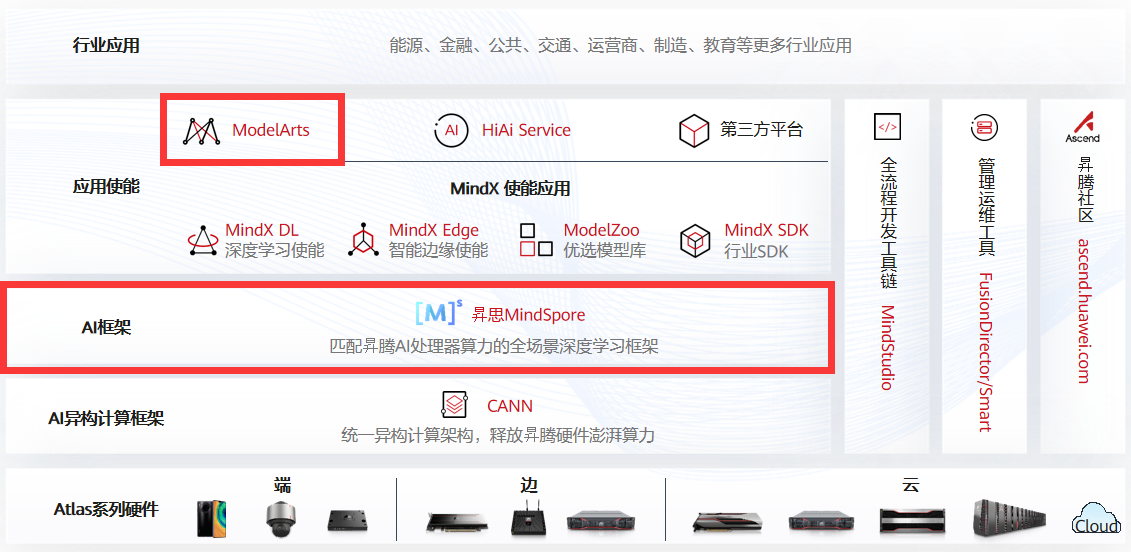
\includegraphics[width=1\textwidth]{figures/mindspore-whole-picture.png}
	\caption{caption:mindspore-whole-picture}
	\label{fig:mindspore-whole-picture}
\end{figure}

MindSpore框架拥有全场景AI计算能力,图\ref{fig:mindspore-ai-architecture}展示了MindSpore全场景AI计算框架架构图,其包含了AI计算所需的各个组件,从软件到硬件,从网络模型、API表达层、编译优化层到底层各种计算资源硬件和其使用框架,均包含在MindSpore中。

\begin{figure}[htbp]
	\centering
	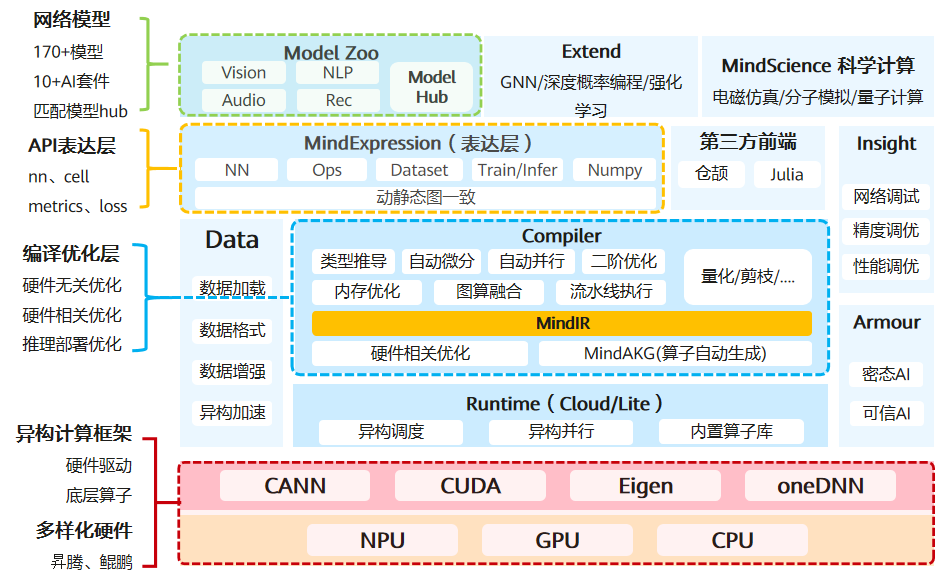
\includegraphics[width=1\textwidth]{figures/mindspore-ai-architecture.png}
	\caption{caption:mindspore-ai-architecture}
	\label{fig:mindspore-ai-architecture}
\end{figure}


MindSpore 架构具有如下特点:
\begin{itemize}
    \item 用户态易用;
    \item 运行态高效;
    \item 部署态灵活;
\end{itemize}

MindSpore 具有如下特性:
\begin{itemize}
    \item 自动并行:通过自动并行机制、数据pipeline处理等手段降低超大模型训练门槛。
    \item AI+科学计算:支持AI+科学计算的高阶/高纬、多范式编程。
    \item 通用计算+DSA:通过图算融合对性能进行优化,自动算子生成技术简化异构( DSA )编程,发挥多样性算力的性能。
    \item 端边云统一的可信架构:解决企业级部署和可信的挑战。
\end{itemize}


MindSpore包含了MindExpress、MindCompiler、MindSpore Runtime、MindData等多个子系统,在实验指导书中不再赘述,有兴趣了解的同学可以参考助教分享的演示文稿。


\subsection{MindSpore安装}

安装过程也与Pytorch的安装类似,具体而言,打开\url{https://www.mindspore.cn/install},选择合适的版本、平台等后,按照网站的指示安装即可。

\begin{figure}[htbp]
	\centering
	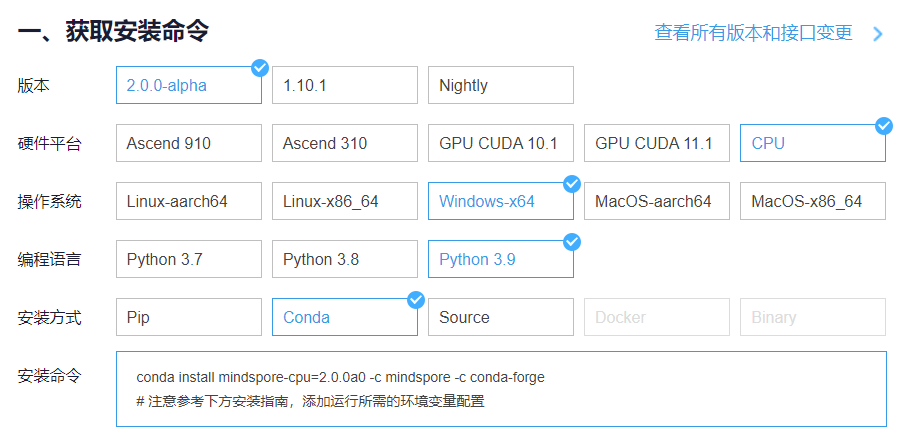
\includegraphics[width=1\textwidth]{figures/mindspore-install.png}
	\caption{caption:mindspore-install}
	\label{fig:mindspore-install}
\end{figure}

\subsection{社区资源}
\begin{itemize}
    \item {\CJKfontspec{HanaMinA}昇}腾开发者社区: \url{https://hiascend.com}
    \item {\CJKfontspec{HanaMinA}昇}腾论坛: \url{https://www.hiascend.com/forum/}
    \item MindSpore开源社区:  \url{https://www.mindspore.cn/}
    \item ModelArts社区:  \url{https://bbs.huaweicloud.com/forum/forum-718-1.html}
    \item Gitee仓库: \url{https://gitee.com/mindspore}
\end{itemize}
